%% Template for SDP report, adapted from mlp_cw2_template, 2018. 

%% Based on  LaTeX template for ICML 2017 - example_paper.tex at 
%%  https://2017.icml.cc/Conferences/2017/StyleAuthorInstructions

\documentclass{article}
\usepackage[T1]{fontenc}
\usepackage{amssymb,amsmath}
\usepackage{txfonts}
\usepackage{microtype}
\usepackage{xspace}
\xspaceaddexceptions{\%}

% Lists with less spacing between items
\usepackage{paralist}

% For figures
\usepackage{graphicx}
\usepackage{subfig} 

% For citations
\usepackage{natbib}

% For algorithms
\usepackage{algorithm}
\usepackage{algorithmic}

% the hyperref package is used to produce hyperlinks in the
% resulting PDF.  If this breaks your system, please commend out the
% following usepackage line and replace \usepackage{mlp2017} with
% \usepackage[nohyperref]{mlp2017} below.
\usepackage{hyperref}
\usepackage{url}
\urlstyle{same}

% Packages hyperref and algorithmic misbehave sometimes.  We can fix
% this with the following command.
\newcommand{\theHalgorithm}{\arabic{algorithm}}


% Set up MLP coursework style (based on ICML style)
\usepackage{mlp2018}
\mlptitlerunning{SDP Demo \demoNumber  Group (\groupNumber)}
\bibliographystyle{icml2017}


\DeclareMathOperator{\softmax}{softmax}
\DeclareMathOperator{\sigmoid}{sigmoid}
\DeclareMathOperator{\sgn}{sgn}
\DeclareMathOperator{\relu}{relu}
\DeclareMathOperator{\lrelu}{lrelu}
\DeclareMathOperator{\elu}{elu}
\DeclareMathOperator{\selu}{selu}
\DeclareMathOperator{\maxout}{maxout}







%% You probably do not need to change anything above this comment

%% REPLACE the details in the following commands with your details
\setGroupNumber{20}
\setGroupName{ENRS}
\setProductName{FInDO}
\setLogoFileName{figs/sdp_logo_placeholder.png}

\begin{document} 

\makeSDPTitle{Project Plan}

% Previous MLP Style Title Layout working. 
% \twocolumn[
    % \mlptitle{\productName: SDP Demo \demoNumber}
    % \centerline{Group \groupNumber: \groupName}
% ]

\begin{abstract} 
%The abstract should first consist of one sentence describing the intended functionality of your system. It should be followed by a few sentences (100--200 words) summarising the main milestones that will bring your project to a successful completion. This should give the reader a clear expectation of what will be achieved throughout the semester.

For those who have reduced mobility, FInDO will be able to deliver them preselected everyday items on trays to locations around the house. The robot will be able to map out the layout of the house and navigate back and forth from the tray cubbies to the user. The user will be able to save delivery locations and FInDO will be able to navigate to those locations with tray in hand (or paw). It will be capable of  storing and retrieving trays in the cubbies. Using image recognition, FInDO will be able to figure out what is in each of the trays for more intuitive instructing. Lastly, it will have an easy to use interface to control this functionality in the form of both an app and support for voice commands.

\end{abstract} 

\section{Goal description} 
%This section should start with a paragraph stating, in simple words, the key idea of your system. Describe the problem in one sentence, and use another sentence to describe your solution.

For people living with reduced mobility moving around the home to get items can be a challenge. To reduce the need for this we propose a robot which can bring household items to the user so they do not have to retrieve them themselves.
\subsection{Relevance of the system} 
%If possible you should then provide evidence that the problem is relevant, by referencing published research that demonstrates a need and / or characterizes a potential market for your system. If appropriate, include reference to existing systems that you are taking as inspiration. You should cite the sources (e.g. \cite{Newell81}) and add the details to the example-refs.bib file so that the full references appears in the bibliography section.

In 2011/12 6.5 million people in Great Britain had some level of impairment to their mobility \cite{disabilitystats}. This shows a large need for such a system, and with the population in the UK aging \cite{agegrowth} this need will increase in the coming years.

We have determined that an App is an appropriate interaction mechanism based on internet usage in the targeted age groups. In 2018 80.2\% of 60-75 year olds had recently used the internet and 43.6\% of those aged over 75 years old had recently done so \cite{webage}. This shows that our choice of using an App to control the robot should be accessible to a large portion of our target market while also retaining the flexibility an App brings.

\subsection{High-level description} 
%You should then provide the description of your problem in terms of functionalities. A common approach in the software industry is to rely on user stories. Internet is full on resources on the topic and you should investigate it.
A typical usage of FInDO will be similar to what follows. The user will select on the app what storage unit they would like to access, and where in the home they are located. FInDO will proceed to move to the relevant storage unit, and pick it up. The storage unit will then be  brought to the user and placed in the location specified. The storage unit will remain in that location as needed. When the user wishes for the storage unit to be returned FInDO will proceed to pick up the unit again and take it back to the  storage area.

\subsection{User Stories}

1.FInDO should be able to identify and collect the correct storage unit. The robot needs to associate items with given storage units and be able to retrieve the correct storage unit when needed.

2. The robot should be able to navigate its way around the home to get to the destination. We intend for the robot to have a mapped version of the flat/house/space it is operating in. With that, the robot should be able to make autonomous decisions on how to get from one place to another. This is useful for the user as this is what makes the robot capable of bringing the items to the user.

3. FInDO should be able to bring storage units to multiple specified locations throughout the home. This gives the user flexibility to be in multiple places in the home rather than having to be in a specific location to have items brought to them. 

4. The robot should be controllable by a mobile/web application. We intend for there to be a mobile/web application that would be used as a way to remotely control the robot. The user should be able to specify a location where they are located and an object they would like to access and have the correct unit brought to them.

5. The robot should have voice activation. We intend for the robot to be activated by voice if the user does not have their phone with them. Saying the words “Fido, fetch me item name to destination!” would activate the robot which would then identify the item in question and take it to the destination.

6. The robot should be able to identify objects placed in storage units so that they can be associated with them. This helps users as they do not have to input the items manually, which would be very inconvinient for many people and be a long process.

\section{Task planning}
%In this section you must provide a detailed plan of the tasks to be completed to achieve your goals. The plan must comprise two levels: first a few milestones that correspond to major achievements in the project, then a detailed list of atomic tasks that must be achieved.

\subsection{Milestones} 
%From the user stories, you should extract the main technical subgoals, i.e., what you need to accomplish to get to the desired final result. For each subgoal you should provide an explicit milestone that states what you should have achieved, by what date, and what evidence you will present to show you have achieved it (e.g. a demonstration of the feature to the experts).

We’ve identified five main subgoals and their respective milestones. For each milestone we have also given the completion evidence that we plan to present as well as when we hope to have the subgoal completed.

A: Locomotion Subgoal:
\begin{enumerate}
\item Milestone: Able to plot a route and navigate around the house from cubbies to saved locations
\item To be completed by Demo 2 (March 30)
\item Evidence: Put drone in pre-mapped demo room, have it navigate from one predefined location to a few others
\end{enumerate}

B: Mapping Subgoal:
\begin{enumerate}
\item Milestone: Able to map house, locate itself in the house, and remap on the fly if new obstacles are added
\item To be completed by Demo 4 (March 30)
\item Evidence: Have drone map demo room and show map to experts. Place new object in room and show live map regeneration. Place drone in random position in demo room and have it mark its position on map.
\end{enumerate}
C: Lifting Subgoal:
\begin{enumerate}
\item Milestone: Able to pick tray out of cubby, raise to present tray to user, and deposit tray back in cubby
\item To be completed by Demo 3 (March 9)
\item Evidence: Have drone remove tray from cubby, lift it up and down, then deposit it back in cubby
\end{enumerate}
D: Communication Subgoal:
\begin{enumerate}
\item Milestone: User can activate bot from app or by voice, instructing it which item to deliver and where to. Bot will be able to recognize what items are on trays through image recognition
\item To be completed by Demo 3 (March 9)
\item Evidence: Instruct bot to do simple locomotion task through app and voice command
\end{enumerate}
E: Image Recognition Subgoal:
\begin{enumerate}
\item Milestone: Bot can recognize item on tray and deliver correct tray when instruction requests specific item
\item To be completed by Demo 4 (March 30)
\item Evidence: Place different items on a tray and have bot correctly identify them
\end{enumerate}


\subsection{Task decomposition} 
Each milestone should then be decomposed into a set of ``atomic'' tasks, taking no more than 20 hours each. Each task should be given a name, a one-sentence-long description, and an estimated time for completion.


You can summarize the tasks in a table, (for instance, table~\ref{tab:sample-table}, using the \verb+table+ environment).

\begin{table*}[h]
\vskip 3mm
\begin{center}
\begin{small}
\begin{sc}
\begin{tabular}{lcccp{3cm}}
\hline
\abovespace\belowspace
Task Name & Subgoal  & Deadline & Dependencies &  Rough description \\
\hline
\abovespace
Mapping house & Mapping & February 3 & N/A & Generate map of house using SLAM \\ \hline
Forklift design & Lifting & February 3 & N/A & Design the parts of the robot that allow it to lift trays. \\ \hline
Cubby design & Lifting & February 3 & N/A & Design an effective stacking and storing system for the trays. \\ \hline
Tray design & Lifting & February 3 & N/A & Design trays that can be stably carried by bot and stored efficiently \\ \hline
Navigation to point & Locomotion & February 24 & Mapping house & Navigate on map to any given point within house \\ \hline
Forklift implementation & Lifting & February 24 & Forklift design & Build forklift and ability to move it up and down. \\ \hline
Cubby implementation & Lifting & February 24 & Cubby design & Build cubby \\ \hline
Tray implementation & Lifting & February 24 & Tray design & Build trays \\ \hline
App interaction & Communication & February 24 & Navigate to point & App can activate and instruct bot \\ \hline
Interact with cubbies & Lifting & March 9 & Cubby imp. Tray imp. Forklift imp. & Able to retrieve and store trays in cubbies \\ \hline
Voice interaction & Communication & March 9 & Navigation to point & Reacts to voice commands through smart home equipment \\ \hline
Continuous map generation & Mapping & March 30 & Navigation to point, Mapping house & Able to remap as it navigates to account for new obstructions \\ \hline
Identify items on trays & Image Recognition & March 30 & Cubby imp. Tray imp. Forklift imp. & Able to recognize what items are on trays through image recognition \\ \hline
\belowspace
\end{tabular}
\end{sc}
\end{small}
\caption{Task decomposition for the system}
\label{tab:sample-table}
\end{center}
\vskip -3mm
\end{table*}

%\begin{figure}[tb]
%\vskip 5mm
%\begin{center}
%\centerline{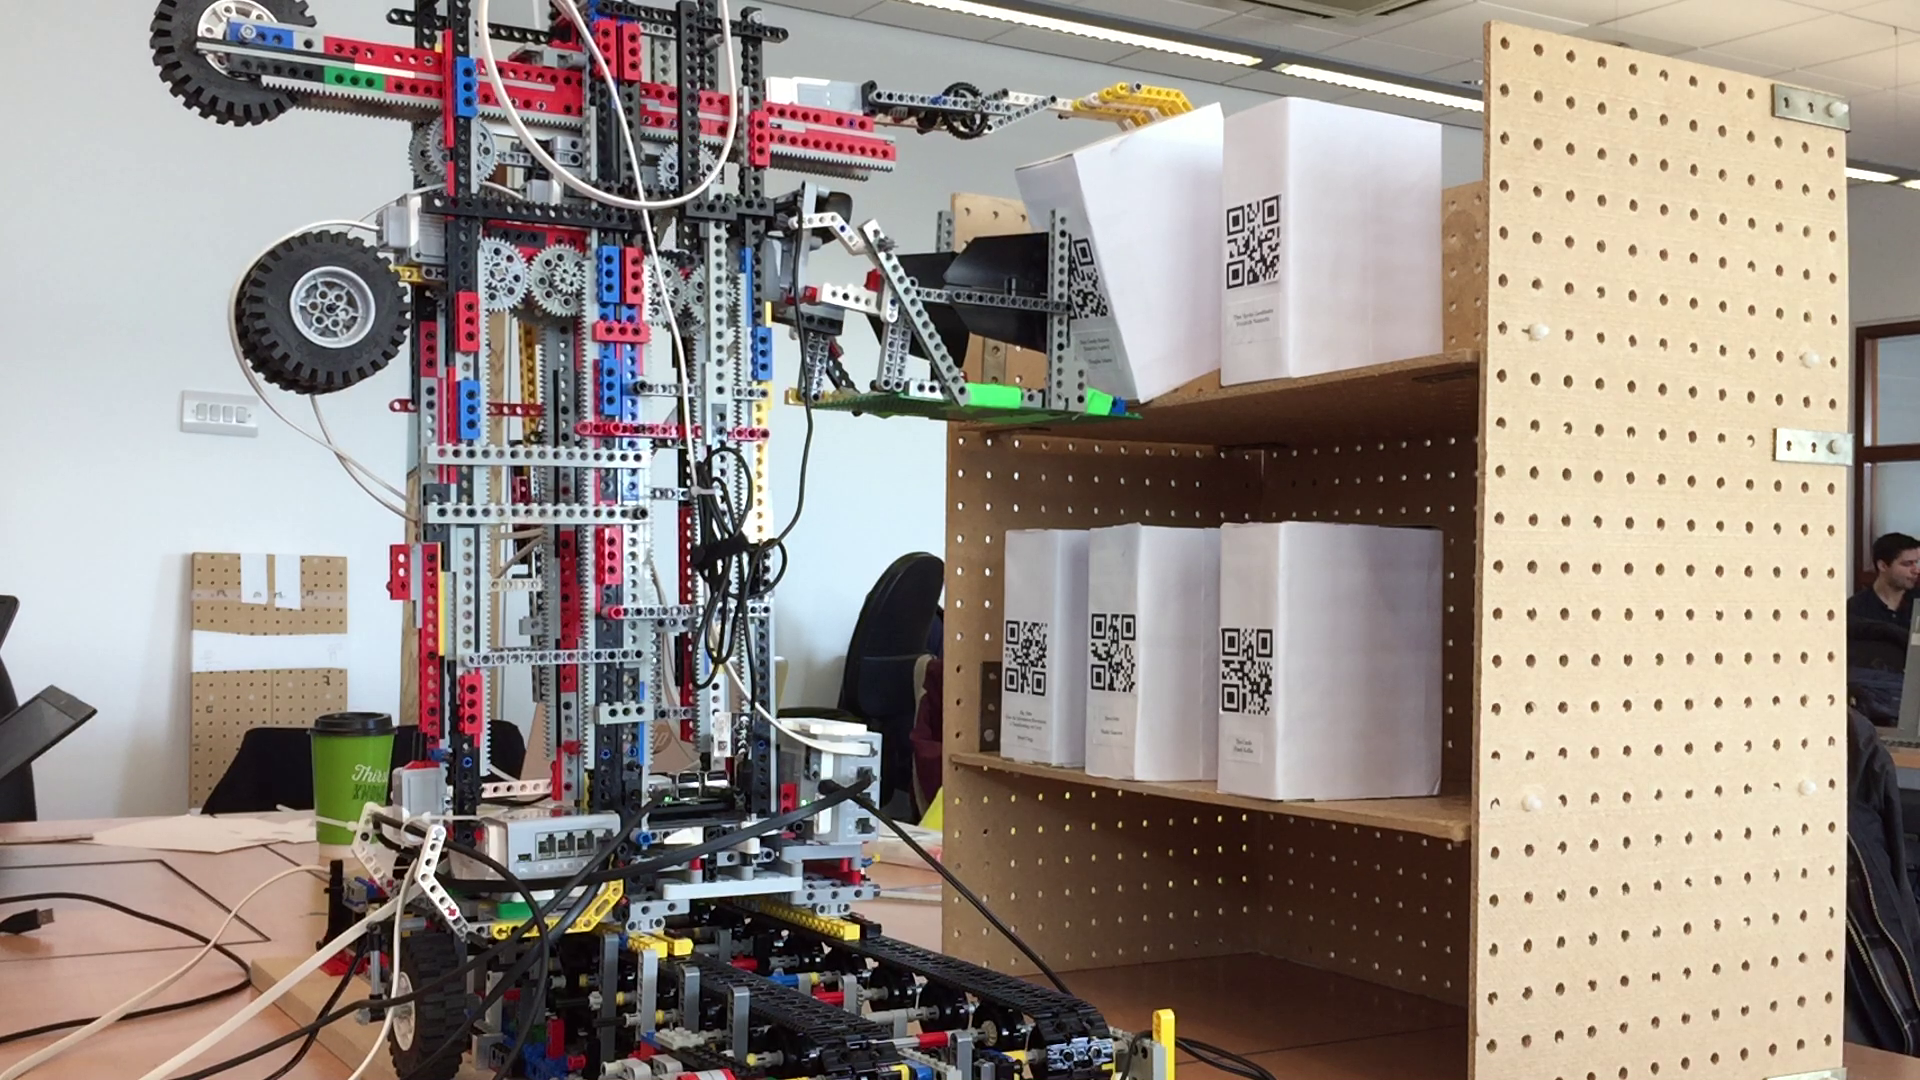
\includegraphics[width=\columnwidth]{figs/crane}}
%\caption{Lego construction: highlight any salient features in the caption}
%\label{fig:sample-fig}
%\end{center}
%\vskip -5mm
%\end{figure} 


\subsection{Resource distribution}
\begin{table*}[h]
\vskip 3mm
\begin{center}
\begin{small}
\begin{sc}
\begin{tabular}{lcccr}
\hline
\abovespace\belowspace
Event (per member) & Estimated Time Consuming(hrs) \\ \hline
\hline
\abovespace
Opening Session & 3 \\ \hline
Workshops & 5 (depends on individuals) \\ \hline
Project pitches & 2 \\ \hline
Group Meetings & 20  \\ \hline
Report Writing & 15 (depends on individuals) \\ \hline
Demonstrations & 10 (depends on school timetable) \\ \hline
Demo Prep & 5 \\ \hline
Individual Working  & 125 \\ \hline
Trade Fair \& Others & 15 \\ \hline
Total & 200 \\ \hline
\belowspace
\end{tabular}
\end{sc}
\end{small}
\caption{Resource distribution}
\label{tab:sample-table}
\end{center}
\vskip -3mm
\end{table*}

Please see Table 2 for time resource distribution

Equipment: 
\begin{itemize}
\item Turtlebot
\item Lego Mindstorms EV3
\item Lego
\item 3D printer
\item Wood/Shelving components 
\item Motors
\item Raspberry Pi
\item Arduino
\item Shelving components
\end{itemize}

Skills: 
\begin{itemize}
\item Front end web development experience
\item Database experience
\item Python
\item Java
\item C++
\end{itemize}
\subsection{Risk assessment} 

Lack of Hardware Experience

The majority of this team are more proficient in software with limited hardware skills. We have identified this weakness and have a team that will focus heavily on hardware. Appropriate resources will be used, including the provided experts, at the early stage of this project in order to allow for a learning curve and any other hidden problems. Also the earlier completion of the hardware will allow the software team to understand the capabilities that they will be dealing with.

Unfeasible Goals

As with something that we want to design we may delve into the unlikely or impossible standards/features that we wish to implement. Realizing that some of our goals may not be possible in the timeframe, we have placed achievable milestones that we wish to complete with this project. This ensures that we will create a working project and will have the flexibility to extend our functionality/usability should we have the resources to spare.

Team Cohesion

There is a lack of experience of working on a large project like this, as such there may be problems in management and effective time allocation of team members. We have split the team into general areas of hardware and software(On robot and App) in order to give a clear focus on their role within the project. Flexibility between areas is also implemented in case extra/less hours are required for certain parts of the project. General meetings will be held regularly and open communication between all team members through slack, github etc, will update the team on the condition of the project. This will allow input from all members and checks in the quality of the product.

Sell Factor

This project will be focusing on a helper bot that works as an aid to those that struggle with getting everyday items. As the audience target market would include the elderly and infirm, we realize the high quality of standard/service that our project must have in order to be recognized as a feasible product. We understand that this would be a tough market to break into and will plan our functionality accordingly with use of provided experts and internet research/statistics.

Lift Mechanism

The lifting mechanism of the turtle bot is critical to this project. Main areas of problems will arise with the balance of the bot and the stability of taking out a tray down to the bot. To combat this the bot should be under the tray that it is using and we will ensure proper caution is given to the planning that will heavily incorporate solutions to these obvious problems. Opinions will be sourced from the technicians at various stages with multiple potential prototypes in order to find an optimal solution.

\section{Group organisation}

To communicate within the team we are using Slack for messaging, to manage the project we will be using Jira. To share code we will be using a central GitHub repository for all of the projects code - using a single repository will ensure all members will have access to the latest version of the entire codebase for reference.

We plan to have meetings 1-2 times per week to check in on progress throughout the team and discuss any issues that need to be resolved. A member of the team will take on the role of chairperson each meeting to keep the meetings on track. 

Members have been split between 3 sub-teams for each of the 3 main areas of the project. Hardware design, software design (Robot side), and software design for the control app. Members have been assigned to these teams based on experience and preference for the relevant tasks the teams will tackle. These teams are not concrete and we anticipate a large degree of flexibility and interworking during the project. Tasks within these sub-teams will be assigned to members based on ability, and current workload from other tasks they have taken on. 

We will be tracking progress using Jira, we will be asking members of the team to update any progress they have made daily. This will allow for early detection of issues with task progress, so members can help troubleshoot and resolve issues. During meetings we will also check the projects overall progress compared to the milestones highlighted early in the document to ensure that we are on track and make changes accordingly.


%% Include any references in a bibliography

\bibliography{example-refs}

\end{document} 

